\chapter{Data and Exploratory Analysis}
\label{sec:data}
% STATUS: first draft (2026-10-05), written from the Phase 1a EDA (Project/EDA/report/eda_report.md) and the Phase 1
% report (Project/docs/phase1_report.md). Numbers are reproducible with `groundone data build|check|shortcut` and the
% EDA scripts. TODO: final pass after the main results; add the training-mix table from the manifest.

GroundOne has to learn and be evaluated on four kinds of decisions: whether a sentence is supported by a document,
whether it is contradicted or merely not mentioned, whether it is acceptable under a stated verification rule, and all
of these for several sentences of the same answer at once. No single public dataset covers all of them. This chapter
describes the four datasets used in the thesis, where they come from, what an exploratory analysis revealed about
them, and how they were turned into training, development and test sets without leakage.

\section{The datasets and their origin}
\label{sec:data:origins}

\paragraph{ANLI.} Adversarial NLI~\cite{nie2020anli} is a natural language inference corpus collected in three rounds
against increasingly strong models: human annotators wrote hypotheses that would fool the model of the round, and
only the successful ones were kept. Premises are short paragraphs, mostly from Wikipedia in rounds 1--2 and from
several genres (news, fiction, spoken text, WikiHow) in round 3. Each pair has a human label among
\emph{entailment}, \emph{neutral} and \emph{contradiction}, which map directly onto \emph{supported},
\emph{not mentioned} and \emph{contradicted}. The corpus has 162{,}865 training pairs and balanced development and
test splits of 3{,}200 pairs each (licence CC BY-NC 4.0~\cite{hf_anli}).

\paragraph{RAGTruth.} RAGTruth~\cite{niu2024ragtruth} contains 17{,}790 answers written by six LLMs (GPT-3.5, GPT-4,
Llama-2 7B/13B/70B and Mistral-7B) in three retrieval-augmented tasks: question answering over three retrieved
passages for MS MARCO questions~\cite{nguyen2016msmarco}, summarisation of news articles
(CNN/DailyMail~\cite{see2017pointer,hermann2015teaching} and recent news), and data-to-text generation from Yelp
business records in JSON~\cite{yelpdataset}. Annotators marked the character spans of each answer that are not
grounded in the context, distinguishing \emph{Conflict} (contradicts the context) from \emph{Baseless Info} (adds
content the context does not contain), each \emph{Evident} or \emph{Subtle}. It is the only dataset of real,
multi-sentence LLM answers over a shared context, which is the setting GroundOne targets (licence MIT).

\paragraph{MiniCheck synthetic data.} The 14{,}395 claim--document pairs released with
MiniCheck~\cite{tang2024minicheck,hf_minicheck_data} were generated with GPT-4 so that verifying a claim requires
combining several sentences of the document. Labels are binary and follow from the construction. They are the
training data of the strongest small baseline, so using them makes the comparison with MiniCheck approximately
data-matched (licence MIT).

\paragraph{LLM-AggreFact.} LLM-AggreFact~\cite{tang2024minicheck,llmaggrefact} aggregates eleven human-labelled
datasets of (document, claim) pairs: summarisation (AggreFact-CNN/XSum~\cite{tang2023aggrefact},
TofuEval-MediaSum/MeetingBank~\cite{tang2024tofueval}), retrieval-augmented and long-form question answering
(RAGTruth~\cite{niu2024ragtruth}, ClaimVerify~\cite{liu2023verifiability}, ExpertQA~\cite{malaviya2024expertqa},
LFQA~\cite{chen2024lfqa}) and fact checking (WiCE~\cite{kamoi2023wice}, REVEAL~\cite{jacovi2024reveal},
FactCheck-GPT~\cite{wang2024factcheckbench}). Its score is the unweighted mean balanced accuracy over the eleven
datasets at a fixed threshold of 0.5. The gating condition of its licence (CC BY-ND 4.0) allows it to be used only
as an evaluation benchmark~\cite{hf_llmaggrefact}; in this thesis it is therefore never used for training, nor for
fitting temperatures, thresholds or model selection.

Table~\ref{tab:data:overview} summarises the differences that matter for the experiments.

\begin{table}[htbp]
\centering
\small
\begin{tabular}{lllll}
\hline
 & ANLI & RAGTruth & MiniCheck synth. & LLM-AggreFact \\
\hline
Claim written by & humans (adversarial) & LLMs & GPT-4 & LLMs and humans \\
Labels from & humans & humans (spans) & construction & humans \\
Label scheme & 3 classes & 4 span types & binary & binary \\
Unit & pair & multi-sentence answer & pair & pair \\
Median document & 73 tokens & 308--685 tokens & 186 tokens & 530 tokens \\
Size & 169{,}265 pairs & 17{,}790 answers & 14{,}395 pairs & 59{,}740 pairs \\
Role & train, dev, test & train, dev, test & train, dev & test only \\
\hline
\end{tabular}
\caption{The four datasets. Document lengths are in Qwen2.5 tokens; RAGTruth's range spans its three tasks.}
\label{tab:data:overview}
\end{table}

\section{Exploratory analysis}
\label{sec:data:eda}

\paragraph{Label balance.} ANLI's development and test splits are exactly balanced across the three classes, while
its training split is skewed towards \emph{neutral} (Figure~\ref{fig:data:anli-labels}). RAGTruth is the opposite:
deriving one label per sentence (a sentence is \emph{contradicted} if it overlaps a Conflict span, \emph{not
mentioned} if it overlaps only Baseless spans, \emph{supported} otherwise), the training split contains 105{,}572
supported, 8{,}077 not-mentioned and 4{,}658 contradicted sentences. Contradictions are concentrated in data-to-text
(77\,\% of Conflict spans); in the QA test split only 0.5\,\% of sentences are contradicted
(Figure~\ref{fig:data:ragtruth}). A three-way evaluation on RAGTruth alone would therefore be uninformative: ANLI
carries the three-way question and the verification rules.

\begin{figure}[htbp]
\centering
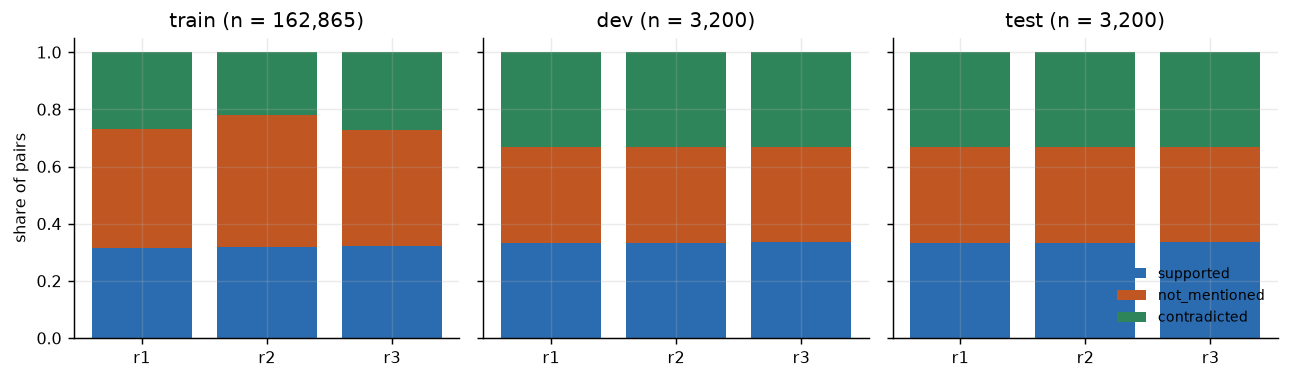
\includegraphics[width=\textwidth]{images/eda/anli_labels.png}
\caption{ANLI label shares per split and round: balanced development and test splits, neutral-heavy training split.}
\label{fig:data:anli-labels}
\end{figure}

\begin{figure}[htbp]
\centering
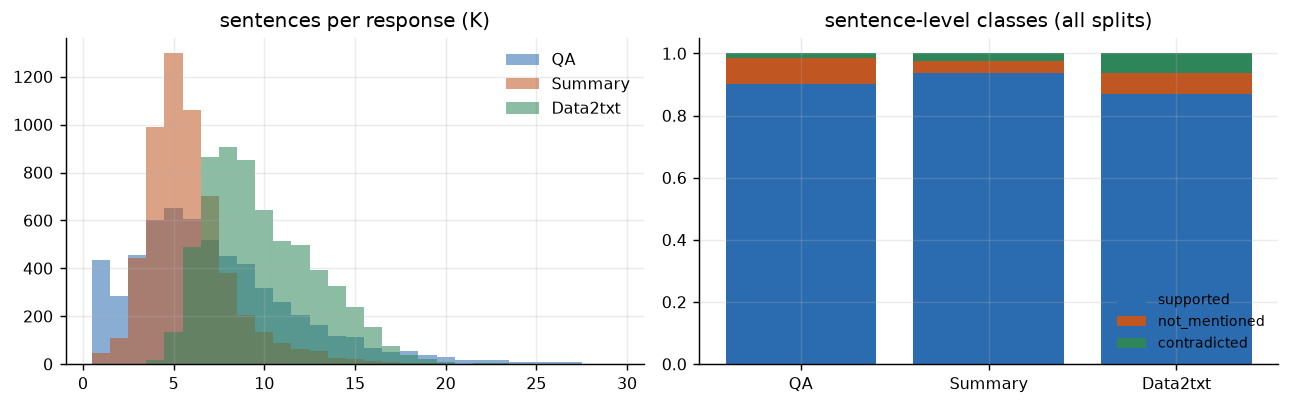
\includegraphics[width=\textwidth]{images/eda/ragtruth_sentences.png}
\caption{RAGTruth at sentence level: number of sentences per answer ($K$) by task, and the share of supported, not
mentioned and contradicted sentences.}
\label{fig:data:ragtruth}
\end{figure}

\paragraph{Sentences per answer.} The median answer has 9 sentences in data-to-text, 6 in QA and 5 in summarisation,
and 45\,\% of the answers have at least 8 sentences. With three questions per sentence, 15 to 27 decisions over the
same context are typical: the regime in which a single-pass, shared-prefix System One is expected to be fastest
(Chapter~\ref{sec:method}).

\paragraph{Lengths.} Documents differ by an order of magnitude across datasets (Figure~\ref{fig:data:lengths}).
For RAGTruth, 22\,\% of the full prompts (context and answer) exceed 1{,}024 tokens but only 1\,\% exceed 2{,}048,
so a training cap of 2{,}048 tokens keeps almost all of it. In LLM-AggreFact, 2.4\,\% of the test documents are
longer, mostly in ClaimVerify and WiCE; at evaluation time they are split into chunks and a claim is considered
supported if any chunk supports it, as in MiniCheck~\cite{tang2024minicheck}.

\begin{figure}[htbp]
\centering
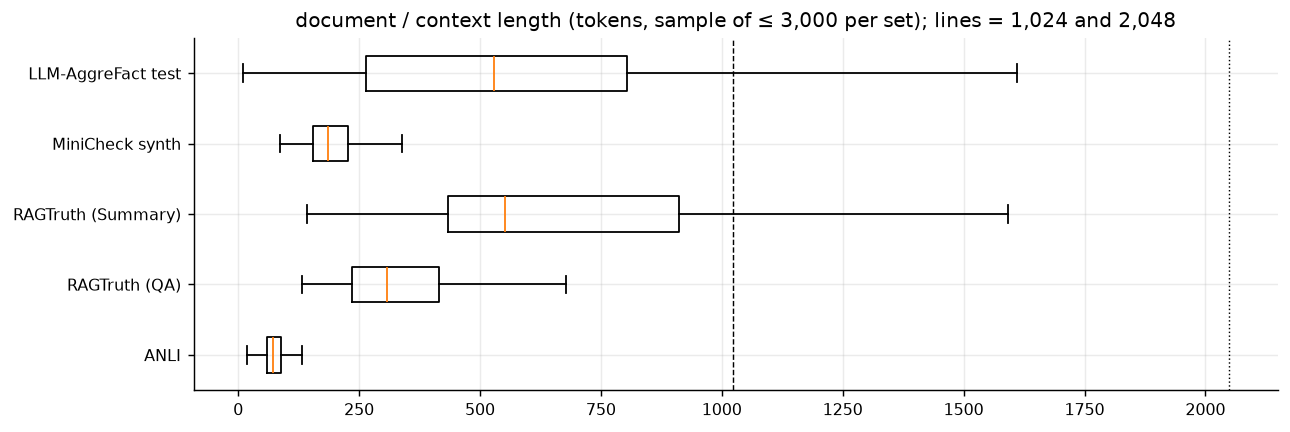
\includegraphics[width=\textwidth]{images/eda/cross_doc_lengths.png}
\caption{Document length across the datasets (sample of up to 3{,}000 documents each); dashed lines at 1{,}024 and
2{,}048 tokens.}
\label{fig:data:lengths}
\end{figure}

\paragraph{A label shortcut in ANLI.} In ANLI's training split, 26\,\% of contradiction hypotheses contain a
negation word, against 8--10\,\% for the other classes. In the development and test splits the pattern is reversed,
a consequence of the adversarial collection (Figure~\ref{fig:data:shortcut}). A bag-of-words classifier that sees
only the claim reaches 0.56 balanced accuracy on held-out training pairs (chance 0.33) but only 0.36 and 0.39 on the
development and test splits. Cues of this kind can be learned from the training data and do not transfer; ANLI's
test split will expose a model that relies on them.

\begin{figure}[htbp]
\centering
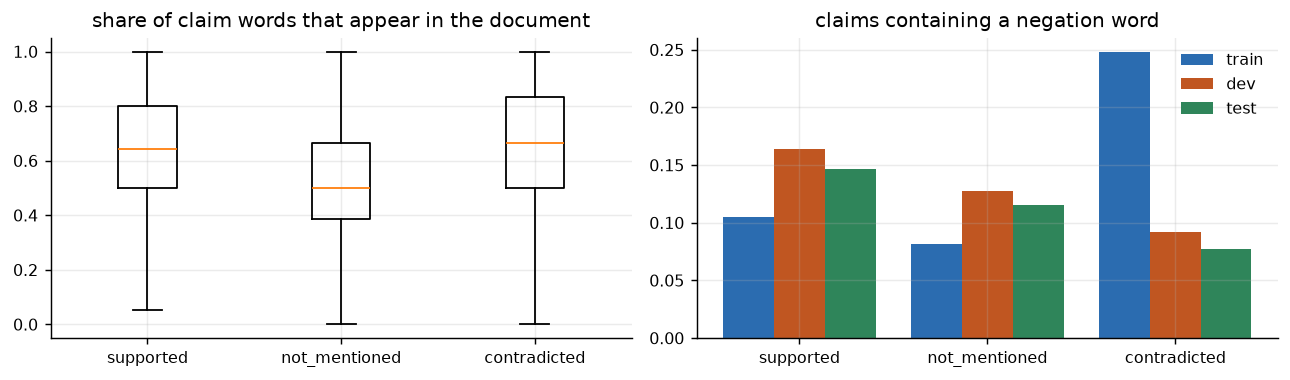
\includegraphics[width=\textwidth]{images/eda/anli_shortcuts.png}
\caption{Surface cues in ANLI: share of claim words found in the document, and share of claims containing a negation,
by class and split.}
\label{fig:data:shortcut}
\end{figure}

\paragraph{LLM-AggreFact's sub-datasets.} Label balance ranges from 23\,\% supported (REVEAL) to 92\,\% (RAGTruth),
which is why balanced accuracy is used (Figure~\ref{fig:data:aggrefact}). In several sub-datasets (REVEAL,
FactCheck-GPT) many negatives are true statements paired with irrelevant evidence: they measure whether a claim is
supported \emph{by this document}, not whether it is true, which is the definition GroundOne adopts. ExpertQA's
labels were given by experts who used their own knowledge, and all published models score between 50 and 61 on it;
it is reported with that caveat. RAGTruth, LFQA, ClaimVerify and ExpertQA are the sub-datasets closest to local RAG
and are also reported as a separate average.

\begin{figure}[htbp]
\centering
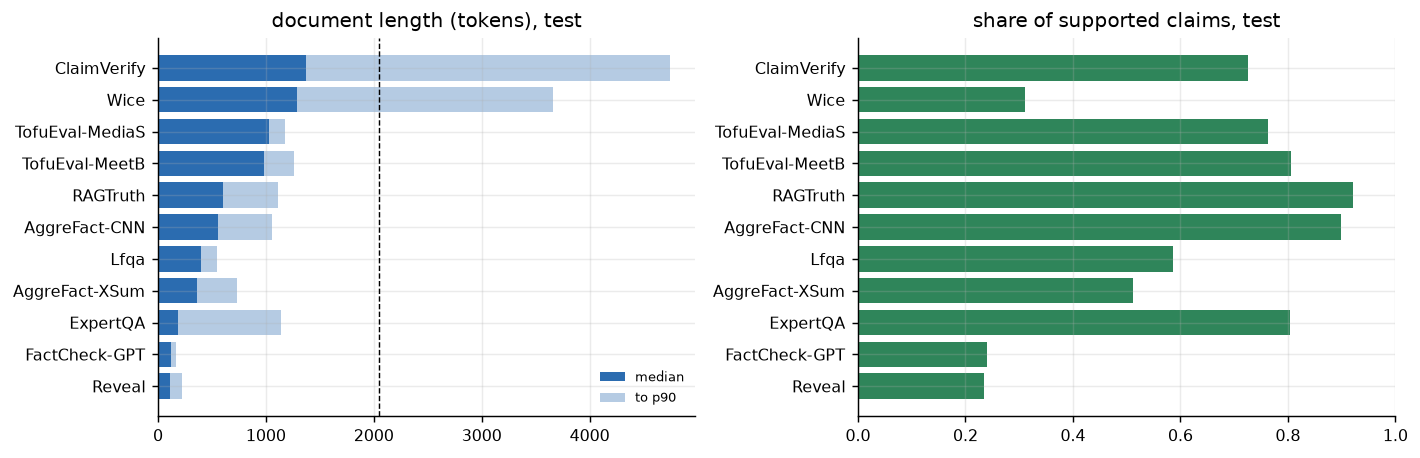
\includegraphics[width=\textwidth]{images/eda/aggrefact_datasets.png}
\caption{LLM-AggreFact test sub-datasets: document length and share of supported claims.}
\label{fig:data:aggrefact}
\end{figure}

\section{Overlaps and leakage}
\label{sec:data:leakage}

Two overlaps were found and both shape how the data is used.

\begin{itemize}
\item \textbf{LLM-AggreFact's RAGTruth sub-dataset is RAGTruth.} Of its 15{,}340 development claims, 14{,}046 are
sentences of RAGTruth's \emph{training} split; of its 16{,}371 test claims, 14{,}942 are sentences of RAGTruth's
\emph{test} split. Training on RAGTruth's training split is therefore safe for LLM-AggreFact's test set, and
RAGTruth's test split and the RAGTruth part of LLM-AggreFact's test set are the same data, reported once. On the
29{,}191 matched sentences, the binary labels derived here from RAGTruth's spans agree with LLM-AggreFact's labels
in 98.6\,\% of cases; all disagreements are sentences we label unsupported and LLM-AggreFact labels supported.
\item \textbf{ANLI reuses premises across splits.} Each premise has about 16 hypotheses, and 98.6\,\% of the
development premises and 98.9\,\% of the test premises also appear in the training split with other hypotheses.
Training pairs whose premise appears in the development or test split are excluded (93{,}480 pairs remain), and the
711 development pairs that share a premise with the test split are removed so that the development split can be
used for calibration.
\end{itemize}

No overlap was found between the MiniCheck data or ANLI and LLM-AggreFact. RAGTruth's own splits share no source
document. A leakage check runs on every dataset build and fails on any shared document or (document, sentence) pair
between training or development data and any test set. On version~1 it found one CNN article used both in RAGTruth's
training split and in LLM-AggreFact-CNN's test split, whose two training sentences were removed.

\section{Usability per experiment and resulting splits}
\label{sec:data:usability}

Table~\ref{tab:data:usability} summarises which dataset serves which experiment.

\begin{table}[htbp]
\centering
\small
\begin{tabular}{p{4.2cm}p{2.3cm}p{2.6cm}p{2.1cm}p{2.3cm}}
\hline
Experiment & ANLI & RAGTruth & MiniCheck synth. & LLM-AggreFact \\
\hline
Binary training & yes (filtered) & yes (rebalanced) & yes & no \\
Benchmark comparable with the literature & secondary & test = AggreFact-RAGTruth & no & \textbf{primary} \\
$K$ decisions per context & synthetic only & \textbf{natural} & no & RAGTruth part only \\
Three-way question & \textbf{primary} & train; test too skewed & no & no \\
Rules in the prompt & \textbf{primary} & mainly data-to-text & no & no \\
Calibration (dev) & yes & dev by source & possible & no (licence) \\
Demo realism & no & QA & no & no \\
\hline
\end{tabular}
\caption{Usability of each dataset for each experiment.}
\label{tab:data:usability}
\end{table}

The resulting dataset version~1 has a training set of 42{,}910 rows for the 0.5B model (ANLI 21{,}000, 7{,}000 per
class; MiniCheck 13{,}990; RAGTruth 7{,}920 rebalanced sentences) and a stratified subset of 10{,}000 rows for the 3B
model. Each row is one question about one sentence: binary-only data gets the \emph{supported} question; three-way
data gets one of the four questions (30\,\% supported, 30\,\% three-way, 15\,\% strict rule, 25\,\% lenient rule).
Development sets come from ANLI (official development split, cleaned), RAGTruth (10\,\% of training sources, by
source document) and MiniCheck (3\,\% of documents). Test sets are ANLI's test split, RAGTruth's test split (19{,}902
sentences in 2{,}700 answers) and LLM-AggreFact's test split (29{,}320 pairs).

% TODO: table of the training mix from data/processed/v1/manifest.json (rows, tokens, labels per question type)
